\section{Hardware Design}
\label{sec:hardware}

Building multiple units for installation in different rooms calls for a repeatable assembly and controls that remain accessible once the display is enclosed. The custom carrier PCB in Fig.~\ref{fig:hardware} brings the ESP32-S3 development board, RTC module, power converter, and HUB12 display connector into one assembly with fixed connections and mounting positions. A separate narrow board carries the AP-mode button and status indicators and connects to the controller through a five-pin cable. This arrangement allows the controls to be positioned independently of the main board, giving users access to network setup and device status from the outside of the enclosure.

\begin{figure*}[t]
\centering
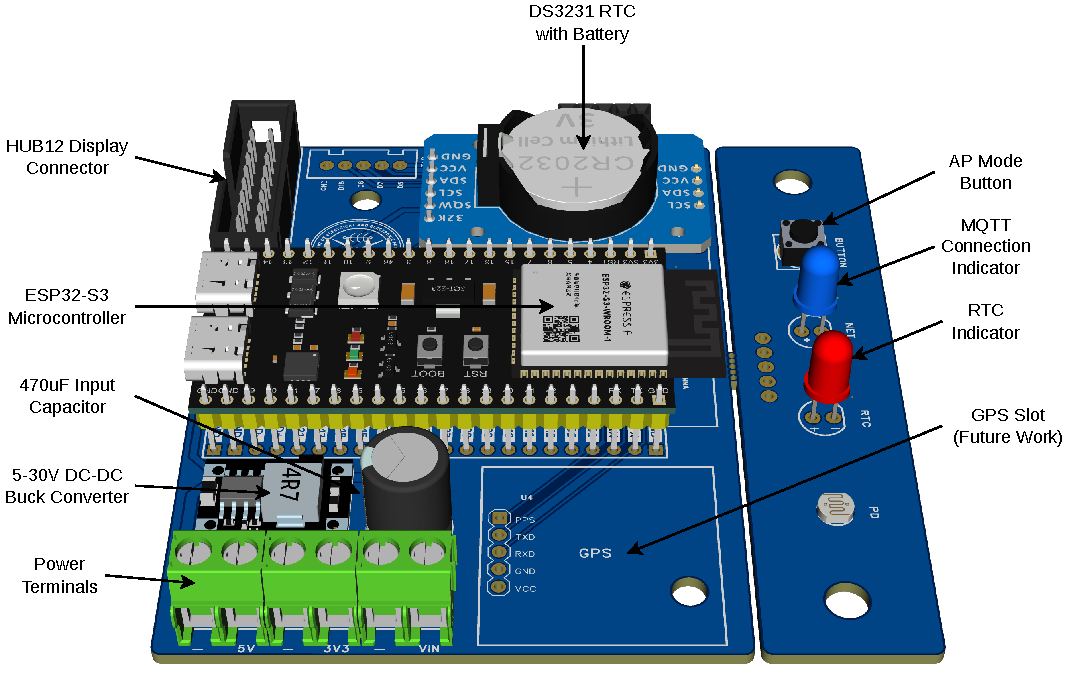
\includegraphics[width=\textwidth]{figs/hardware.pdf}
\caption{Custom controller and user-interface boards, showing the display connection, battery-backed RTC, power stage, and local controls. The GPS slot is reserved for future expansion.}
\label{fig:hardware}
\end{figure*}

The deployed units use two chained $32 \times 16$ P10 LED panels, forming a $64 \times 16$ display. Large digits occupy most of the available height during timekeeping and countdown operation, while longer notices scroll across the same surface. The limited resolution encourages a simple presentation of large characters and animations, with detailed configuration handled through the web dashboard. The HUB12 driver also supports horizontal chaining beyond two panels, allowing wider displays to be built for other installations. Adding panels increases the space available for content while retaining the same 16-pixel height.

Power arrangements can also vary between installations. The board uses a DC--DC buck converter configured for a 5~V output, allowing a higher-voltage DC adapter to supply the required rail. Where a regulated 5~V supply is already available, the converter can be omitted and the bypass connection populated. Screw terminals provide connections for VIN, 5~V, and 3.3~V, while a 470~$\mu$F capacitor across VIN and ground provides input bulk capacitance. These options allow the same PCB to accommodate different supply arrangements.

A DS3231 RTC connected over I$^2$C maintains the local time reference, with a backup battery preserving time while the main supply is disconnected. When power returns, the controller can read the current time before network synchronization becomes available. Together with schedules retained in flash, this provides the hardware basis for the restart behavior described in the \nameref{sec:system_overview} section.